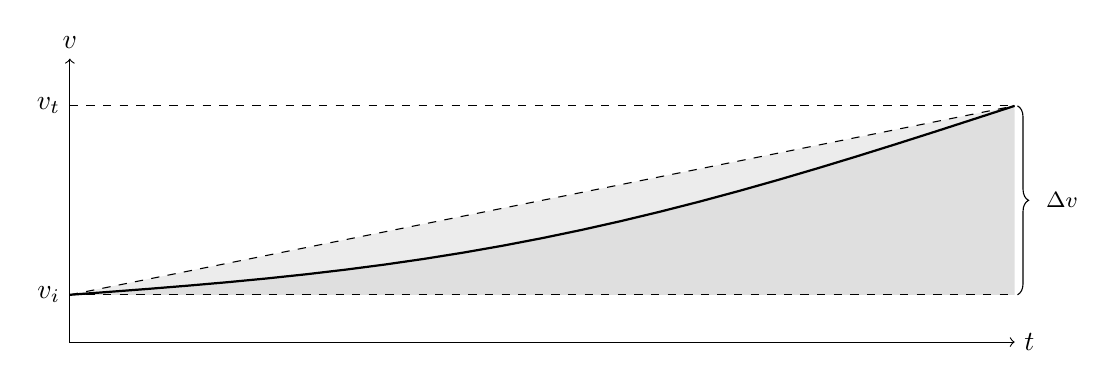
\begin{tikzpicture}[scale=12]

\def\YOffset{0.05}
\def\LinearCoef{0.2}
\def\NonlinearCoef{-0.04}
\pgfmathsetmacro{\InitialTempo}{\YOffset}
\pgfmathsetmacro{\TargetTempo}{\YOffset + \LinearCoef}
\pgfmathsetmacro{\PlotHeigth}{2 * \YOffset + \LinearCoef}
\pgfmathsetmacro{\CenterTempo}{\YOffset + 0.5 * \LinearCoef}

% Draw axes
\draw [<->] (0, \PlotHeigth) node (yaxis) [above] {$v$}
	|- (1,0) node (xaxis) [right] {$t$};

% Position change
\path[fill=gray!50,opacity=.5,domain=0:1]
(0, \InitialTempo) --
plot (\x,
{
	\YOffset +
	\LinearCoef * \x +
	\NonlinearCoef * sin(pi * \x r)
}) --
(1, \InitialTempo) --
cycle;

% non-linear position change
\path[fill=gray!50,opacity=.3,domain=0:1]
(0, \InitialTempo) --
plot (\x,
{
	\YOffset +
	\LinearCoef * \x +
	\NonlinearCoef * sin(pi * \x r)
}) --
cycle;

% line for linear tempo change
\draw[dashed]
(0, \InitialTempo) --
(1, \TargetTempo);

% actual function
\draw[thick,domain=0:1]
plot (\x,
{
	\YOffset +
	\LinearCoef * \x +
	\NonlinearCoef * sin(pi * \x r)
});

% Initial tempo
\draw[dashed]
(0, \InitialTempo) node[left] {$v_i$} -|
(1, \InitialTempo);

% Target tempo
\draw[dashed]
(0, \TargetTempo) node[left] {$v_t$} -|
(1, \TargetTempo);

% Tempo change
\draw [decorate,decoration={brace,mirror,amplitude=4pt,raise=1pt},yshift=0pt]
	(1, \InitialTempo) -- (1, \TargetTempo)
	node [black,midway,xshift=0.6cm] {\footnotesize $\Delta v$};

% TODO add legend
%\node at (0, -0.05) {$\Delta b_{v_b}$};
%\node at (0, -0.10) {$\Delta b$};

\end{tikzpicture}